\subsection{Kostenschätzung (Total Cost of Ownership)}
\label{subsection_kostenschatzung_TCO}
Neben der Organisation und Durchführung des Projekts bildet die Schätzung der Kosten im Vorfeld eine weitere wichtige Säule des Projektmanagements. Eine möglichst ganzheitliche und realistische Erfassung aller potentiell entstehenden Kosten ist dabei notwendig, um die Entscheidung für oder gegen ein Projekt anhand fundierter Informationen treffen zu können.

Das Total-Cost-Of-Ownership-Konzept wurde im Rahmen einer Studie der Gartner Group zur vollständigen Erfassung der direkten und indirekten Kosten eines PC-Arbeitsplatzes entwickelt. Das Ergebnis der Studie hat dabei gezeigt, dass nur ca. 20\% der Gesamtkosten tatsächlich auf die direkten Anschaffungskosten von Hard- und Software entfallen. Der Großteil der entstehenden Kosten wird folglich durch den Einführungsprozess neuer Systeme und den langfristigen Betrieb selbiger verursacht. Der Einsatz der TCO-Methode kann demnach dabei helfen, ein Bewertungsobjekt mit allen zugehörigen, kostenverursachenden Aspekten zu erfassen und zu bewerten.\footnote{\cite{hansen_business_2009}}

Die Tatsache, dass es sich bei dem untersuchten Studienobjekt lediglich um einen “wenig komplexen” PC-Arbeitsplatz handelt, lässt vermuten, dass bei Einführung komplexer Systeme (z.B. Dokumentenmanagement) der Anteil der Anschaffungskosten über den gesamten Lebenszyklus des Systems weiter schrumpft, während beispielsweise Inbetriebnahme, Wartung und Schulung wesentlich mehr Kosten verursachen. Dieser Zusammenhang verdeutlicht die Wichtigkeit der ganzheitlichen Kostenbetrachtung und rechtfertigt den Einsatz des TCO-Konzepts, welches es zum Ziel hat, den Vollständigkeitsgrundsatz der Kostenrechnung\footnote{\cite{grob_einfuhrung_2004}} zu erfüllen.

Grundsätzlich wird im Rahmen der TCO-Aanalyse zwischen direkten und indirekten, bzw. budgetierten und nicht-budgetierten, Kosten unterschieden. In die Kategorie der direkten Kosten fallen dabei alle Investitionen, die zur Beschaffung und Bereitstellung der IT-Komponente notwendig sind. Die Bezeichnung als budgetierte Kosten liegt darin begründet, dass selbige einem konkreten Bereich (z.B. Hochschulrechenzentrum bei Anschaffung eines neuen Servers) zugeschrieben werden können. Im Gegensatz dazu handelt es sich bei indirekten Kosten um Ausgaben, die außerhalb des Bereichs auftreten, der die direkten Kosten zu tragen hat, wodurch sie keinem konkreten Budget zugeschrieben werden können. Eine generische Übersicht der direkten und indirekten Kategorien zeigt Abbildung \ref{fig_generische_kostenarten} \footnote{\cite{hansen_business_2009}}.

\begin{figure}[h!]
	\centering
	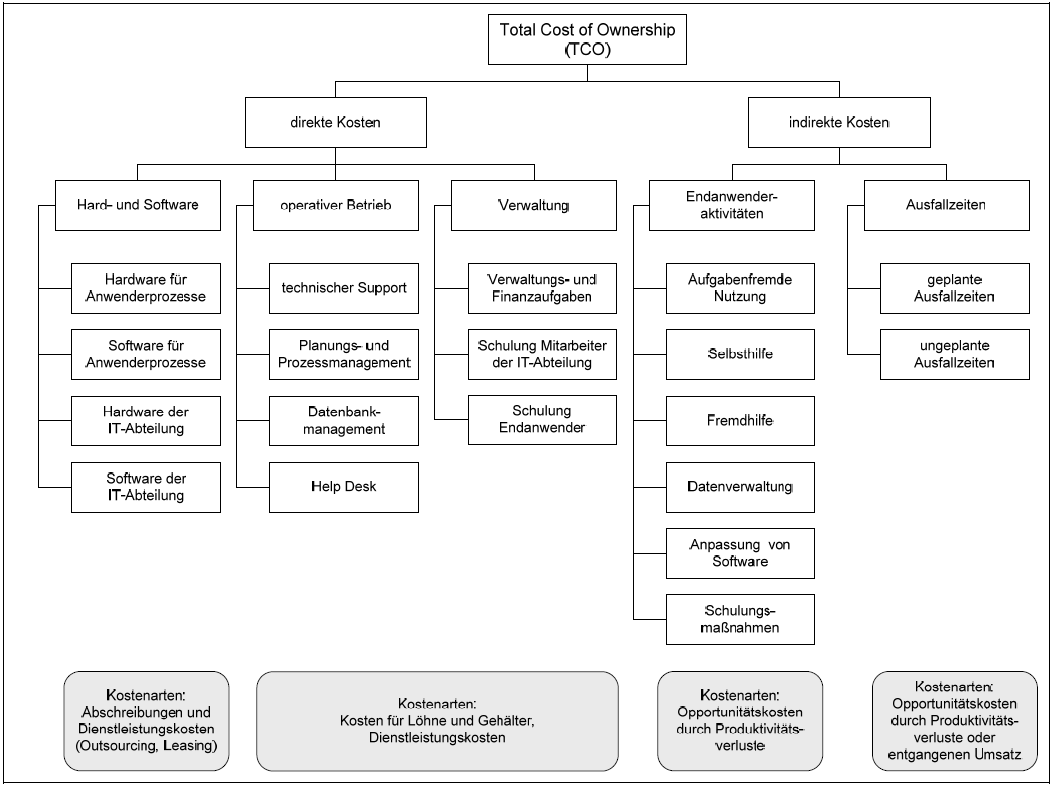
\includegraphics[width=10cm]{kapitel/gruppe4_2/bilder/generische_kostenkategorien}
	\caption{generische Kostenkategorien und -arten, nach Hansen}
	\label{fig_generische_kostenarten}
\end{figure}

Während die im Diagramm dargestellten direkten Kosten auch direkt in der IT-Abteilung anfallen und nachvollziehbar, beziehungsweise durch angemessenen Aufwand berechenbar, sind, entstehen die indirekten Kosten in der Regel durch Endanwender und deren “unsachgemäße Nutzung” der bereitgestellten Infrastruktur. Dies ist theoretisch bereits dann der Fall, wenn ein Mitarbeiter einen anderen Mitarbeiter bei der Lösung von IT-Problemen unterstützt, obwohl dies nicht seine eigentliche Aufgabe ist. Durch diese Arbeiten außerhalb seines Zuständigkeitsbereichs werden die eigentlichen Kernaktivitäten des Mitarbeiters vernachlässigt, wodurch seine Produktivität sinkt. Dieser Produktivitätsverlust wird durch sogenannte Opportunitätskosten abgebildet und als indirekten Kosten erfasst.

Die Erhebung der Informationen, die notwendig sind, um indirekte Kosten beziffern zu können, kann sich jedoch als äußerst schwierig und zeitaufwendig herausstellen. Aufgrund fehlender formalisierter Techniken zur Erfassung eben dieser Positionen, empfiehlt die Gartner Group den Einsatz von Befragungen und Fokusgruppen, was neben dem bereits erwähnten, hohen zeitlichen Aufwand, außerdem zu Problemen hinsichtlich der Validität der Daten führen kann.\footnote{\cite{hansen_business_2009}}

Ferner besteht die Gefahr, dass durch die Berücksichtigung von Opportunitätskosten der in Kapitel \ref{subsection_projektmanagement_hochschule} beschriebene, notwendige Austausch und Kontakt zwischen verschiedenen Arbeitsgruppen und Fachbereichen stark eingeschränkt wird. Deshalb sollte in diesem speziellen, nicht-industriellen, Fall einer Hochschule auf die initiale Berücksichtigung der indirekten Kosten verzichtet werden. Im späteren Projektverlauf, nachdem das Zusammenspiel aller Akteure etabliert und gefestigt ist, muss jedoch versucht werden, diese Daten zu evaluieren und in die Kalkulation mit einzubeziehen.

Eine beispielhafte Kalkulation auf Grundlage der TCO-Methode der Gartner Group wird in Kapitel \ref{subsubsection_dokusystem_alfresco} durchgeführt. Als unterstützende Software zur Berechnung dient die kostenlose Anwendung TCO-Tool.\footnote{\url{http://sourceforge.net/projects/tcotool/}}